\documentclass[a4paper, 11pt, notitlepage]{article}
\addtolength{\hoffset}{-1cm}
\addtolength{\textwidth}{2cm}
\usepackage[utf8]{inputenc}
\usepackage[frenchb]{babel}
\usepackage[T1]{fontenc}

\usepackage{multicol}
\usepackage{listings}
\usepackage{pdfpages}
\usepackage{hyperref}

\usepackage{color}
\definecolor{lightgray}{rgb}{.9,.9,.9}
\definecolor{darkgray}{rgb}{.5,.2,.2}
\definecolor{purple}{rgb}{0.65, 0.12, 0.82}
\definecolor{brown}{RGB}{140, 0, 0}


\lstnewenvironment{java}
                  {\lstset{
                      language=Java,
                      breaklines=true,
                      showstringspaces=false,
                      commentstyle=\color{red},
                      stringstyle=\color{darkgray},
                      identifierstyle=\ttfamily,
                      keywordstyle=\color{blue},
                      basicstyle=\footnotesize,
                     escapeinside={(*}{*)},
                      frame=single,
                      numbers=left,
                      %xleftmargin=0.08\textwidth
                    }
                  }
                  {}


%%%%%%%%%%%%%%%%%%%%%%%%%%%%%%%%%%%%%%%%%%%%%%%%%%%%%%%%%%%%%%%%%%%%%%%%%%%%%%

\title{
  \huge Rapport de projet \\
  \huge CPS : River City Ransom\\
}
\author{
  Béatrice CARRE \\
  Steven VAROUMAS \\
  \\
}

\begin{document}
\maketitle
\section*{introduction}
Méthodologie pour la conception et l’implémentation de
trusted components

1 Analyse : spécifications algébriques (cours 2)

2 Conception : par contrat à partir des spécifications (cours 3 et 4)

3 Implémentation : garantie vis-à-vis des contrats

Conception par contrat : vérification « légère » en ligne (self-testing)





%%%%%%%%%%%%%%%%%%%%%%%%%%%%   Problème   %%%%%%%%%%%%%%%%%%%%%%%%%%%%


\section{Problème}
petite intro ?

\subsection{Specification}
Le but de la spécification est de reconnaître les éléments logiques d’un programme à partir d’une
définition du jeu River City Ransom.

problèmes d’interprétation personnelle

combler le manque d’éléments

rester cohérents

importante notion de référentiel pour chaque service

représentation d’une liste difficile

représentation de la notion de temps difficile


\subsection{Tests}
Décrire et implémenter les tests pour le respect du contrat.

Pour n conditions sur chaque opération => (2 à $\sim 6)^n$ tests!
Pour chaque argument de méthode, il faut trouver les valeurs à tester.
Si booléen, il suffit de tester avec true et false.
Mais si entier float string etc, il est impossible de tester toutes
les valeurs. Il faut donc sélectionner les valeurs les plus
pertinentes à tester, qui sont en général les valeurs juste avant et
après les limites d'intervales de tests.
Par exemple :

Schéma à insérer ?

Théorie : tous les tests réussissent signifierait que nous avons une application sans bug...

Réalité : il faut aussi que l’implémentation respecte ce qui est
demandé, et toutes les valeurs ne sont pas testées, il est donc
impossible d'être sûrs.


\subsection{Implémentation par contrat}
développer les services et conditions soulevés, en respectant le
squelette étudié.






%%%%%%%%%%%%%%%%%%%%%%%%%%%%   Solution   %%%%%%%%%%%%%%%%%%%%%%%%%%%


\section{Solution}
petite intro ?

\subsection{Specification}
choix d'implementation :

 ramasser => 3 méthodes différentes

 1 objet par bloc => jeter un objet que sur bloc vide

 action gangster => commande aléatoire

 ramasser un perso = équipé comme un objet donc invisible

 argent n’est pas un objet équipé  => peut se récolter autant que l’on
          veut, même si équipé de quelque chose

 Les blocs sont en 2D au sol, mais les personnages peuvent sauter sur
   le troisième axe.

 observateur estVisible() pour afficher ou non des gangsters/persos


\subsection{Tests}
Nous n'avons malheureusement pas fait tout les tests.

Idéalement : pour chaque méthodes, pour chaque valeur : 

\subsection{Implémentation par contrat}


%%%%%%%%%%%%%%%%%%%%%%%%%%%%   CCL  %%%%%%%%%%%%%%%%%%%%%%%%%%%%%%

\section*{CCL}
























%%%%%%%%%%%%%%%%%%%%%%%%%%%%   ANNEXE   %%%%%%%%%%%%%%%%%%%%%%%%%%%%%%

\newpage
\pagestyle{empty}
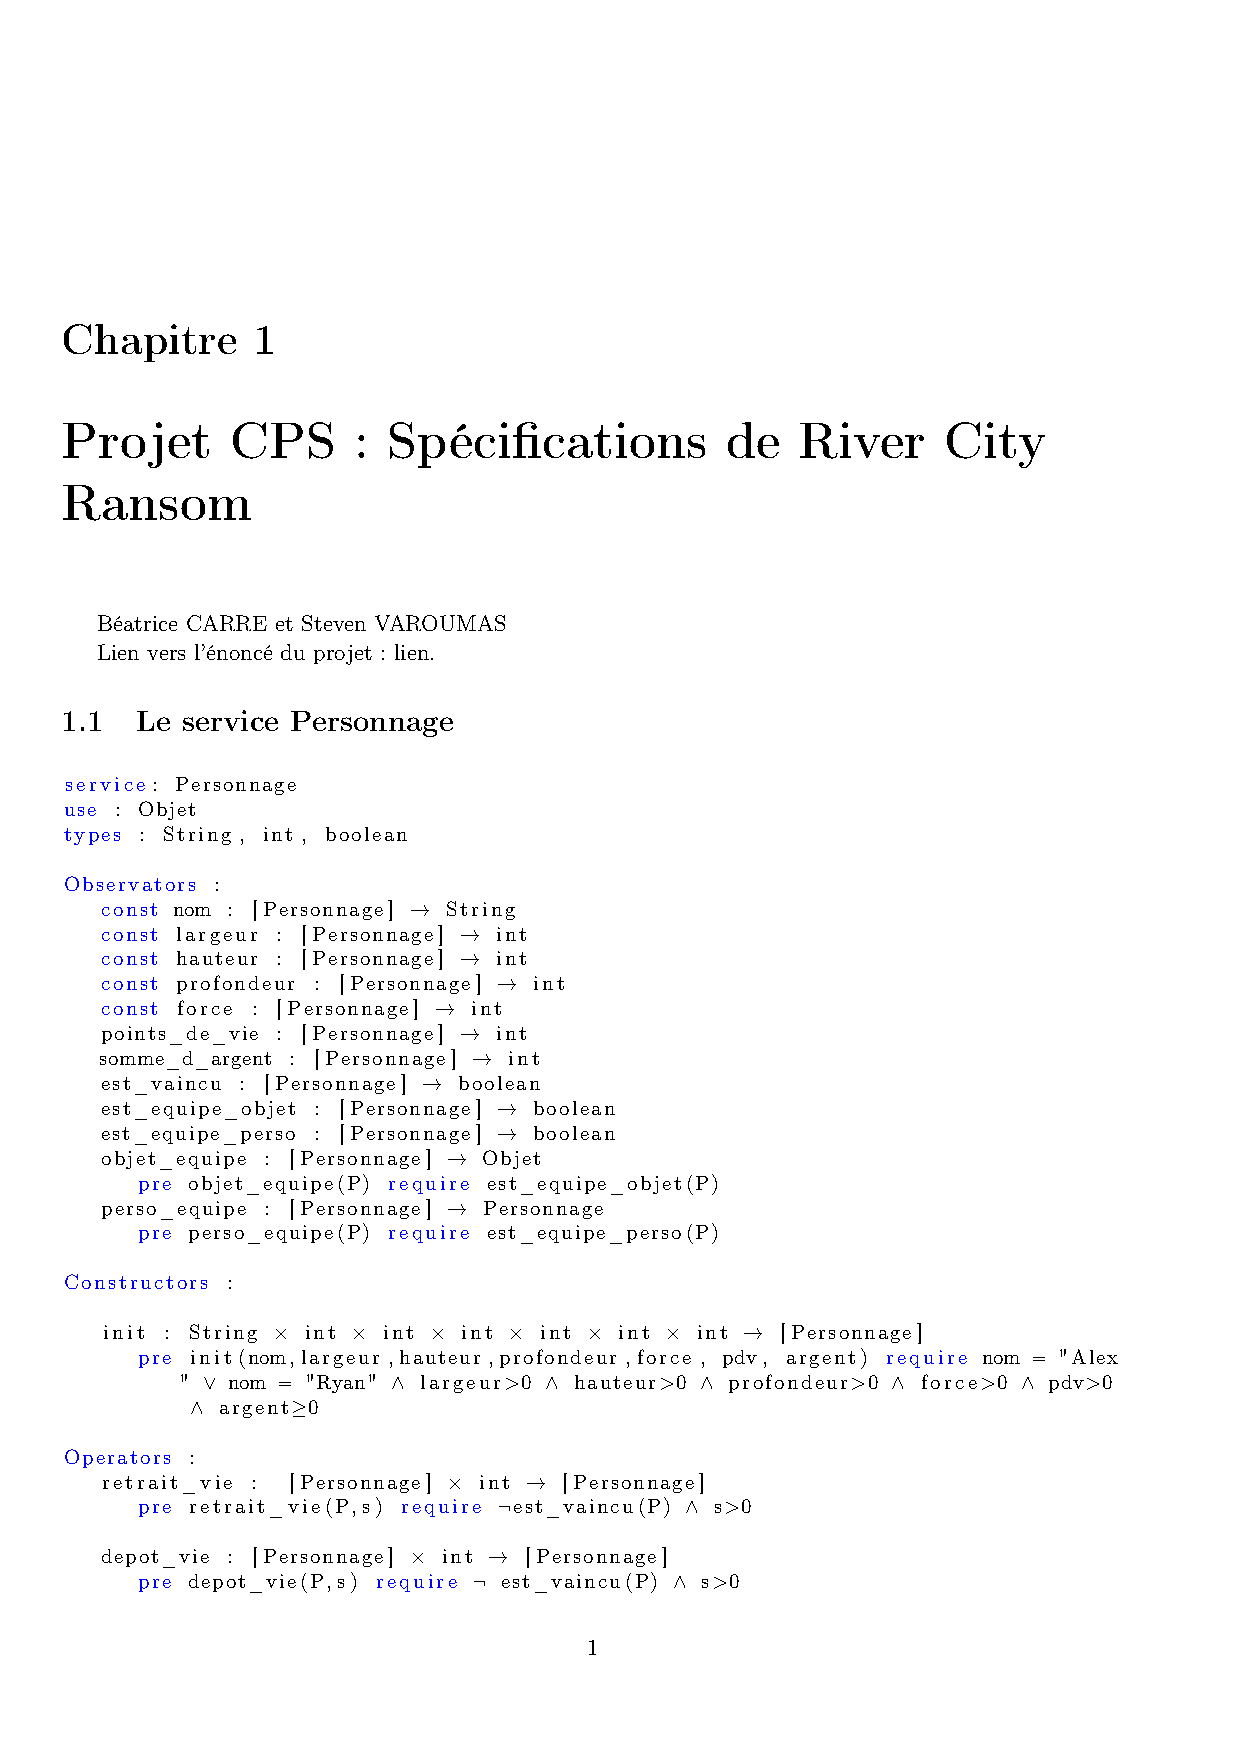
\includepdf[pages={-},pagecommand={},offset=2.cm 1cm]{../Spec/spec.pdf}

\newpage
\pagestyle{empty}
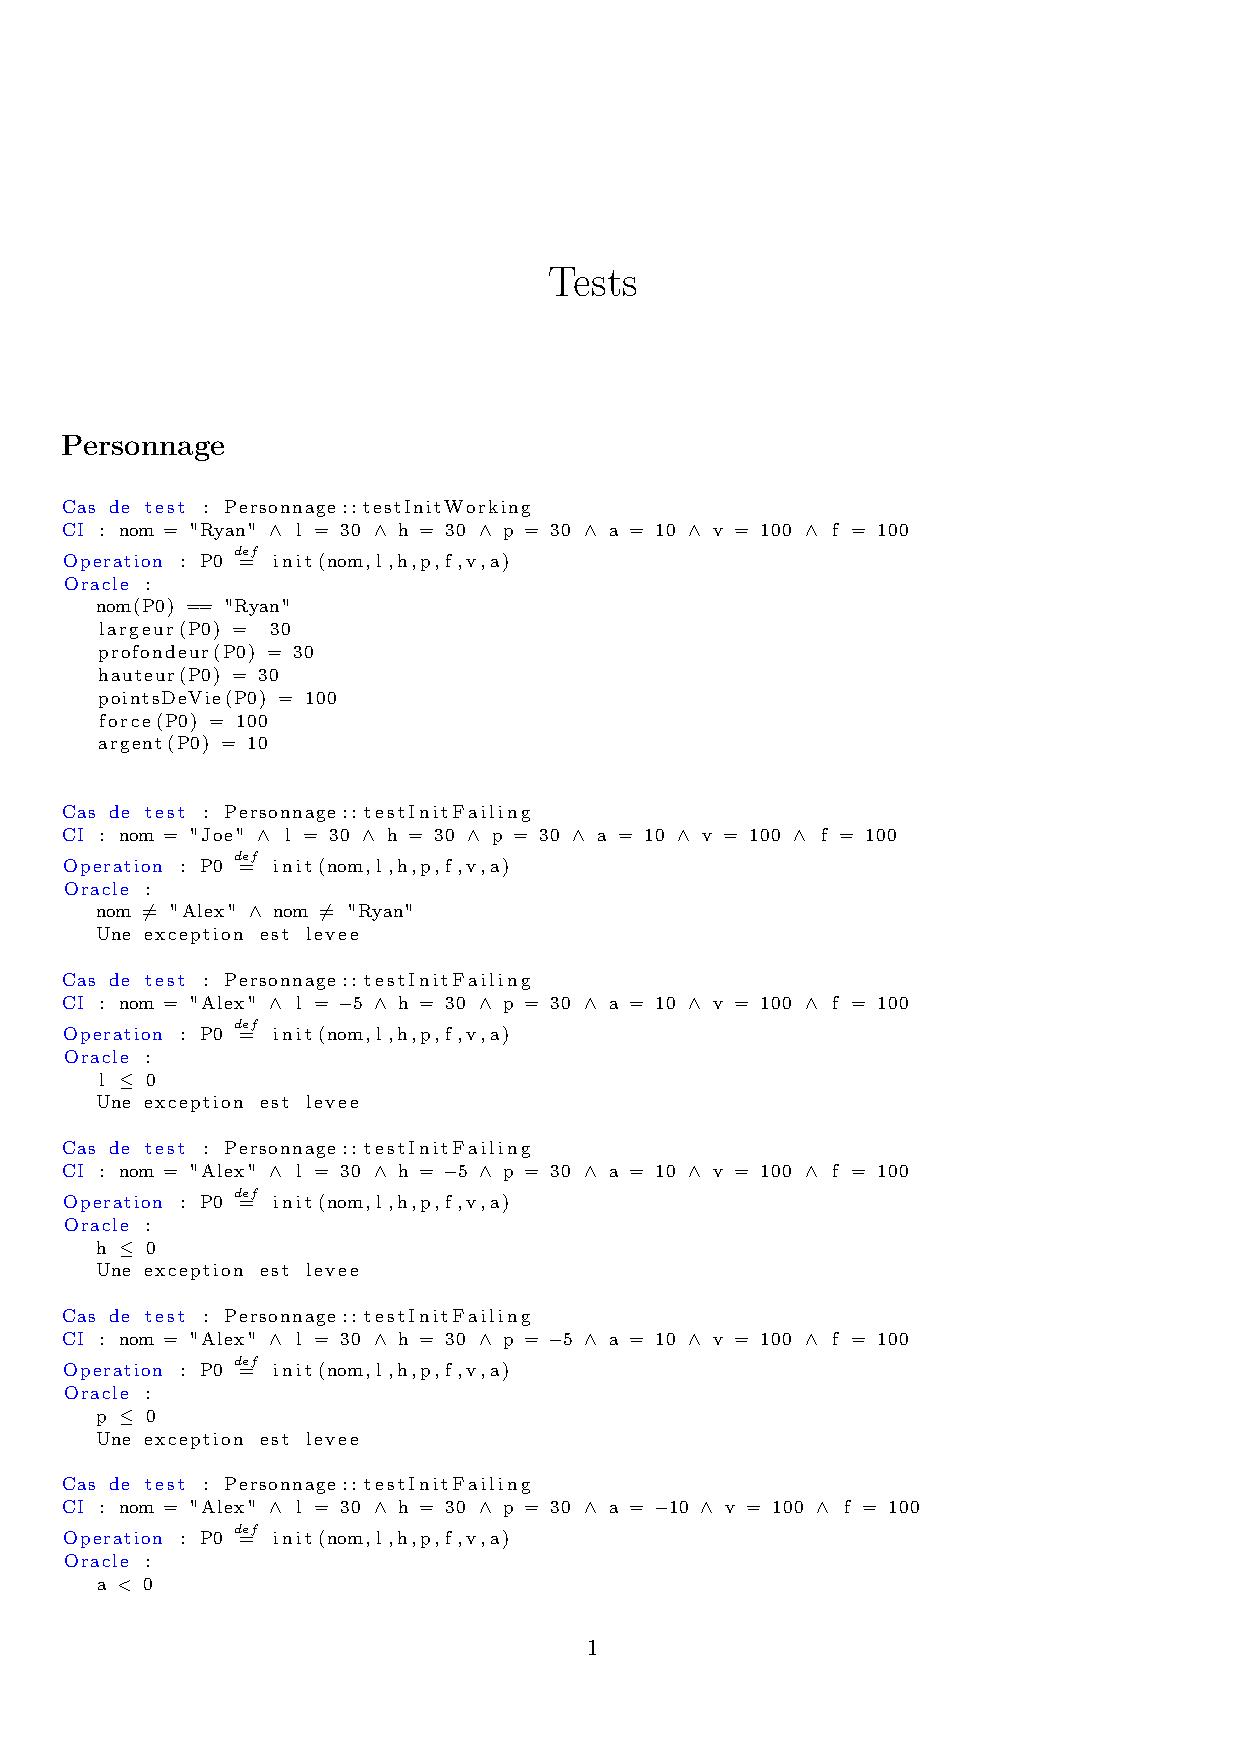
\includepdf[pages={-},pagecommand={},offset=2.cm 1cm]{../Tests/tests.pdf}
\end{document}
